% Created 2017-04-01 Sat 14:32
\documentclass[presentation]{beamer}
\usepackage[utf8x]{inputenc}
\usepackage[T1]{fontenc}
\usepackage{fixltx2e}
\usepackage{graphicx}
\usepackage{longtable}
\usepackage{float}
\usepackage{wrapfig}
\usepackage{rotating}
\usepackage[normalem]{ulem}
\usepackage{amsmath}
\usepackage{textcomp}
\usepackage{marvosym}
\usepackage{wasysym}
\usepackage{amssymb}
\usepackage{hyperref}
\tolerance=1000
\usepackage{minted}
\usetheme{metropolis}
\setbeamertemplate{frame footer}{\color{lightgray}Jeroen Bruijn, Ruud Hendrikx, Elisa Achterberg \& Erwin Rooijakkers - Vegan en Verder}
\metroset{block=fill}
\usetheme{default}
\author{Erwin Rooijakkers, Jeroen Bruijn, Ruud Hendrikx \& Elisa Achterberg}
\date{01-04-2017}
\title{Vegan en Verder}
\hypersetup{
  pdfkeywords={},
  pdfsubject={},
  pdfcreator={Emacs 25.1.1 (Org mode 8.2.10)}}
\begin{document}

\maketitle

\begin{frame}[label=sec-0-1]{Agenda}
\begin{itemize}
\item Dierenleed
\item Marketing
\item Meditation session
\item Gezondheid
\item Verder
\end{itemize}
\end{frame}

\section{Dierenleed}
\label{sec-1}

\begin{frame}[label=sec-1-1]{Animal Rights filmt mishandeling van varkens in slachthuis Tielt (23 maart 2017)}
\url{https://www.animalrights.nl/animal-rights-filmt-mishandeling-van-varkens-slachthuis-tielt}
\end{frame}

\begin{frame}[label=sec-1-2]{Earthlings}
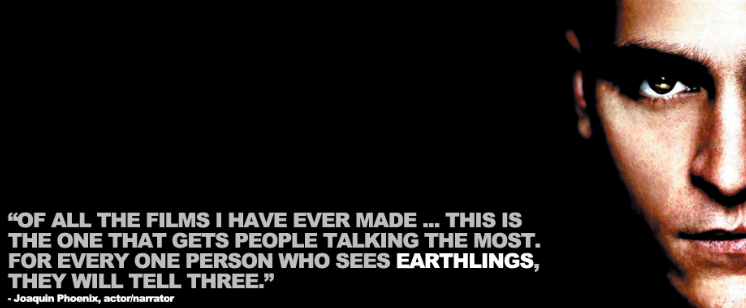
\includegraphics[width=.9\linewidth]{../images/earthlings.png}

\begin{alertblock}{Earthlings}
\url{https://youtu.be/ms7yoerGaPU?list=PLv7whYPHSlwTVb06qz0XrrLikH40cGdhs}
\end{alertblock}
\end{frame}

\begin{frame}[label=sec-1-3]{Melk?}
\begin{alertblock}{DAIRY IS F**KING SCARY! The industry explained in 5 minutes}
\url{https://youtu.be/UcN7SGGoCNI}
\end{alertblock}
\end{frame}

\begin{frame}[label=sec-1-4]{Eieren?}
\begin{alertblock}{What's Wrong With Eggs? The Truth About The Egg Industry}
\url{https://youtu.be/utPkDP3T7R4}
\end{alertblock}
\end{frame}

\begin{frame}[label=sec-1-5]{Biologisch? Organisch?}
\begin{alertblock}{Verschil tussen biologisch en scharrel}
\url{https://www.bio-plus.nl/consument/faq/antwoorden/wat-is-het-verschil-tussen-biologisch-en-scharrel/}
\end{alertblock}
\end{frame}

\begin{frame}[label=sec-1-6]{Biologisch? Organisch?}
\begin{alertblock}{An Unnatural Lifespan}
\url{http://newinfographic.com/wp-content/uploads/2013/09/slaughtering-animals-unnatural-life-span.jpg}
\end{alertblock}
\end{frame}

\section{Marketing}
\label{sec-2}

\section{Meditation session}
\label{sec-3}

\section{Gezondheid}
\label{sec-4}

\begin{frame}[label=sec-4-1]{Anatomie}
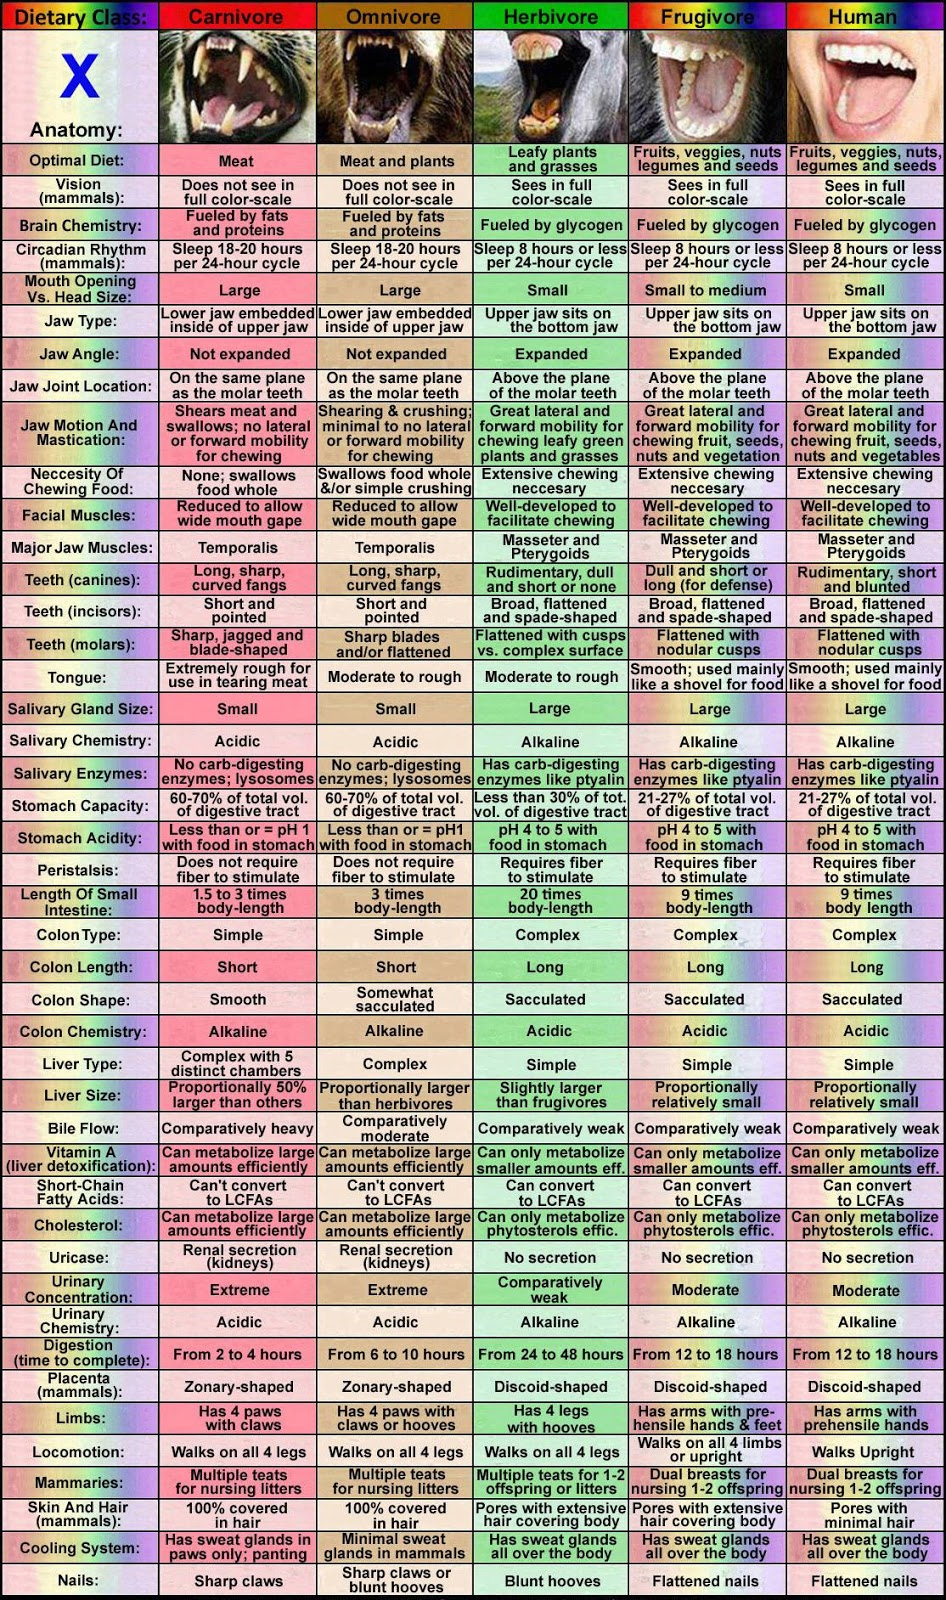
\includegraphics[width=.9\linewidth]{../images/anatomy.jpeg}
\end{frame}

\begin{frame}[label=sec-4-2]{Forks Over Knives}
\begin{quotation}
"The feature film Forks Over Knives examines the profound claim that most, if not all, of the degenerative diseases that afflict us can be controlled, or even reversed, by rejecting animal-based and processed foods."
\end{quotation}

\begin{alertblock}{Forks Over Knives}
\url{https://youtu.be/cgTnd3QPiBY}
\end{alertblock}
\end{frame}

\begin{frame}[label=sec-4-3]{Verder}
\begin{itemize}
\item \url{https://youtu.be/pmAYUf3aemg} (Gary Yourofsky)
\end{itemize}
\end{frame}
% Emacs 25.1.1 (Org mode 8.2.10)
\end{document}
